\documentclass[onecolumn, letter, 11pt]{article}

\usepackage{fourier}
\usepackage[utf8]{inputenc}
\usepackage[sumlimits]{amsmath}
\usepackage{graphicx}
\usepackage[spanish]{babel}
\usepackage{amsfonts}
\usepackage{amssymb}
\usepackage{amsthm}
\usepackage{geometry}

\geometry{left=2.5cm,right=2.5cm,top=2.5cm,bottom=2.5cm}


\title{Examen rápido No. 8}
\author{Inteligencia Artificial, curso 2018-1\\ \textsc{Julio Waissman Vilanova}}
\date{}


\begin{document}

\maketitle

\section{Una red sencillita}

De acuerdo a la siguiente red bayesiana, realiza lo que se pide

\begin{center}
  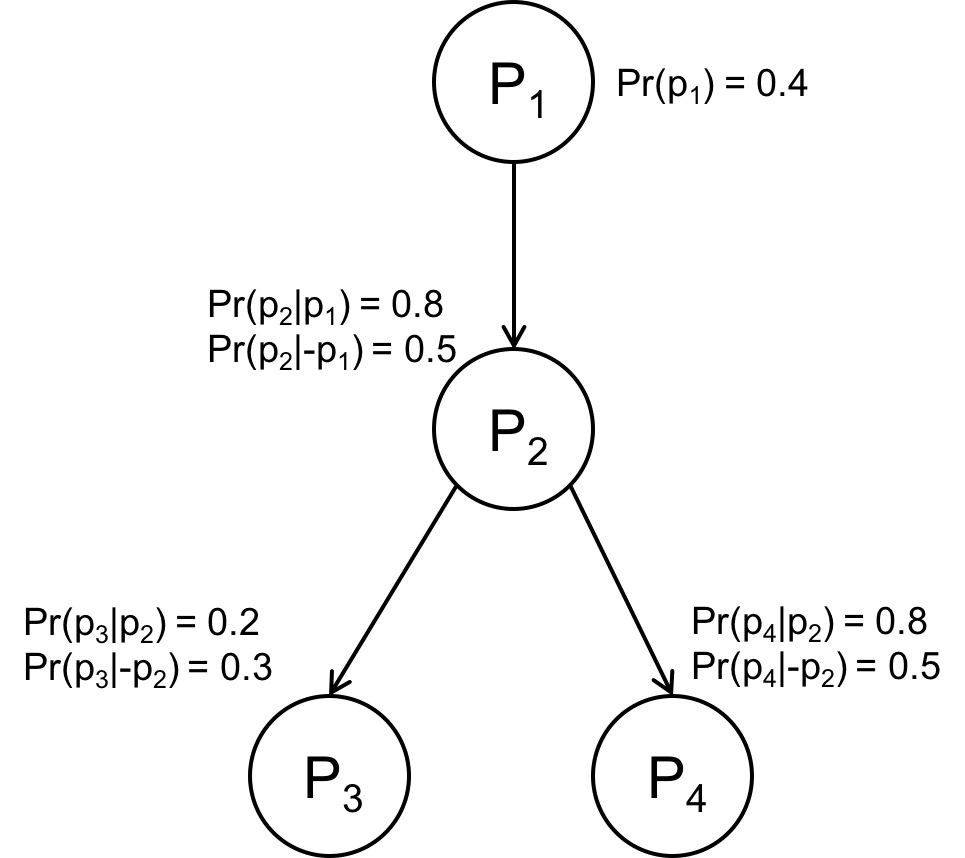
\includegraphics[width=0.5\textwidth]{bayes_leve.png}
\end{center}

\vspace{1cm}

\begin{enumerate}
\item Calcula $\Pr(-p_3)$:
\item Calcula $\Pr(p_2|p_3)$:
\item Calcula $\Pr(p_1|p_2, -p_3)$:
\item Calcula $\Pr(p_1|-p_3, p_4)$:
\end{enumerate}

\newpage
\section{Una red menos sencillita}

De acuerdo a la siguiente red bayesiana, realiza lo que se pide

\begin{center}
  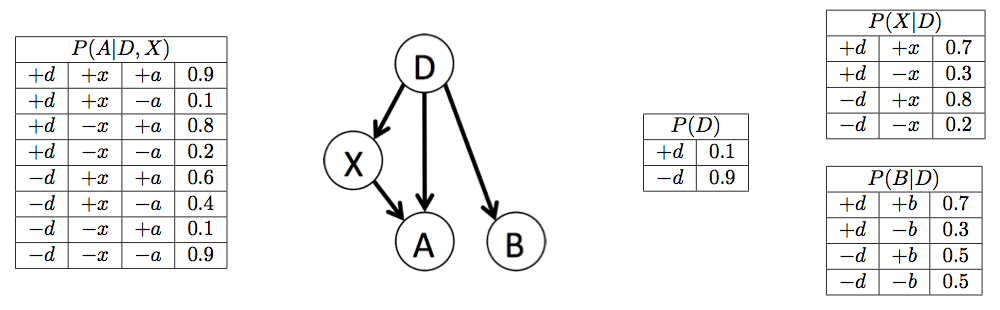
\includegraphics[width=\textwidth]{rb_infe.png}
\end{center}

\begin{enumerate}
\item Calcula $\Pr(+d, +a)$:
\item Calcula $\Pr(-d, +a)$:
\item Calcula $\Pr(+d| +a)$:
\item Calcula $\Pr(+d| +b)$:
\item Calcula $\Pr(+d)$:
\end{enumerate}


\end{document}
